%================================================
% TASK 2.2
%================================================
\section{Task 2.2: StdDev of Amount by SKU-Month with Percentile Threshold}

\subsection{Phân tích truy vấn}
Task 2.2 được phụ trách bởi Nguyễn Hồ Anh Tuấn (23120185). Mục tiêu của truy vấn là xét từng nhóm cặp \texttt{(SKU, month)}, tìm các đơn hàng có số lượng khuyến mãi đủ lớn dựa theo ngưỡng phân vị động của chính nhóm đó, sau đó tính độ lệch chuẩn tổng thể của giá trị \texttt{Amount} trên tập các đơn hàng được giữ lại. Hai mức phân vị bắt buộc là P90 và P80.

Đơn vị lọc ở đây không phải là giá trị đơn hàng \texttt{Amount}, mà là số lượng khuyến mãi của từng đơn hàng. Cột \texttt{promotion-ids} được tách ra theo dấu phẩy, loại bỏ khoảng trắng thừa ở mỗi thành phần, bỏ qua các thành phần rỗng và đếm tất cả các mã khuyến mãi còn lại. Các chương trình khuyến mãi do Amazon phát hành vẫn được tính như khuyến mãi thông thường theo yêu cầu đề bài. Nếu cột \texttt{promotion-ids} mang giá trị null hoặc rỗng, số lượng khuyến mãi \texttt{promo\_count} của đơn hàng được đặt mặc định là 0.

Với mỗi nhóm \texttt{SKU-month}, chương trình tính hai ngưỡng động: \texttt{p90\_thresh} và \texttt{p80\_thresh}. Một đơn hàng được xem là hợp lệ cho mức P90 nếu \texttt{promo\_count >= p90\_thresh}; tương tự, hợp lệ cho P80 nếu \texttt{promo\_count >= p80\_thresh}. Ngưỡng này được tính toán riêng biệt cho từng nhóm cụ thể, hoàn toàn không sử dụng một ngưỡng chung cho toàn bộ tập dữ liệu.

Độ lệch chuẩn tổng thể được tính toán bằng hàm \texttt{stddev\_pop}, tức là độ lệch chuẩn tổng thể với bậc tự do bằng 0:
\[
    \sigma = \sqrt{\frac{\sum_{i=1}^{N}(x_i-\mu)^2}{N}}
\]
Nếu sau khi thực hiện lọc theo phân vị mà nhóm đó có ít hơn 2 đơn hàng, kết quả độ lệch chuẩn của nhóm sẽ được đặt mặc định là \texttt{0.0}. Quy tắc này giúp tránh việc diễn giải sai lệch cho các nhóm chỉ còn lại 0 hoặc 1 đơn hàng hợp lệ sau khi lọc.

Dữ liệu đầu ra được ghi dưới dạng một tệp Parquet duy nhất tại \texttt{data/output/Task\_2-2.parquet} với cấu trúc như sau:
\begin{table}[H]
\centering
\begin{tabular}{ll}
\toprule
\textbf{Cột} & \textbf{Ý nghĩa} \\
\midrule
\texttt{SKU} & Mã SKU của sản phẩm \\
\texttt{month} & Tháng theo định dạng \texttt{yyyy-MM} \\
\texttt{p90\_stddev\_approx} & Độ lệch chuẩn Amount khi dùng ngưỡng phân vị gần đúng P90 \\
\texttt{p90\_stddev\_exact} & Độ lệch chuẩn Amount khi dùng ngưỡng phân vị chính xác P90 \\
\texttt{p80\_stddev\_approx} & Độ lệch chuẩn Amount khi dùng ngưỡng phân vị gần đúng P80 \\
\texttt{p80\_stddev\_exact} & Độ lệch chuẩn Amount khi dùng ngưỡng phân vị chính xác P80 \\
\bottomrule
\end{tabular}
\caption{Định nghĩa schema tệp đầu ra Task\_2-2.parquet}
\label{tab:task2_2_schema}
\end{table}

\subsection{Phân rã thành các bước cơ bản}
Tệp mã nguồn của phần này là \texttt{src/Task\_2-2/source/Task2\_2.scala}. Toàn bộ lời giải sử dụng Spark Structured APIs bằng Scala, tuyệt đối không sử dụng các chuỗi truy vấn Spark SQL dạng thô.

\begin{enumerate}
    \item \textbf{Đọc dữ liệu CSV và chọn các cột cần thiết.} Chương trình đọc tệp dữ liệu \texttt{data/input/Amazon Sale Report.csv} có dòng đầu chứa tiêu đề, giữ lại các cột \texttt{SKU}, \texttt{Date}, \texttt{promotion-ids}, \texttt{Amount}. Cột \texttt{Amount} được chuyển kiểu sang \texttt{DoubleType}; các dòng thiếu thông tin \texttt{SKU}, thiếu ngày tháng hoặc không thể chuyển đổi giá trị \texttt{Amount} sẽ bị loại bỏ để đảm bảo tính hợp lệ cho phép tính độ lệch chuẩn sau này.
    \item \textbf{Chuẩn hóa định dạng tháng.} Cột \texttt{Date} được phân tích cú pháp bằng nhiều định dạng phổ biến như \texttt{M/d/yyyy}, \texttt{MM-dd-yy}, \texttt{M/d/yy}. Sau khi chuyển đổi thành kiểu ngày hợp lệ, chương trình tạo cột tháng \texttt{month = date\_format(parsed\_date, "yyyy-MM")}.
    \item \textbf{Tính số lượng khuyến mãi của đơn hàng} (\texttt{promo\_count}). Cột \texttt{promotion-ids} được tách theo dấu phẩy, loại bỏ khoảng trắng ở mỗi mã khuyến mãi và lọc bỏ các mã rỗng. Số lượng mã hợp lệ còn lại là \texttt{promo\_count}; nếu cột mang giá trị null hoặc rỗng thì mặc định đặt bằng 0.
    \item \textbf{Tạo DataFrame cơ sở.} DataFrame \texttt{baseDf} chỉ giữ lại các cột thông tin tối giản gồm \texttt{SKU}, \texttt{month}, \texttt{promo\_count}, \texttt{amount\_val}. DataFrame này được lưu tạm vào bộ nhớ (\texttt{cache()}) vì cả hai phương pháp tính phân vị gần đúng và chính xác đều sẽ tái sử dụng lại tập dữ liệu này.
    \item \textbf{Tính toán ngưỡng phân vị gần đúng} (\texttt{approxThresholds}). Gom nhóm theo cặp \texttt{SKU, month} và tính toán các ngưỡng phân vị P90 và P80 thông qua hàm \texttt{percentile\_approx(promo\_count, p, 10000)}. Ngưỡng này sau đó được liên kết ngược lại với DataFrame cơ sở \texttt{baseDf} để tiến hành lọc lấy các đơn hàng thỏa mãn.
    \item \textbf{Tính toán ngưỡng phân vị chính xác} (\texttt{exactThresholds}). Chương trình sử dụng hàm cửa sổ với cấu trúc \texttt{partitionBy("SKU", "month").orderBy(promo\_count)} để gán số thứ tự dòng \texttt{row\_number}. Với mỗi nhóm gồm có $N$ đơn hàng, vị trí phân vị chính xác được xác định bằng phương pháp thứ hạng gần nhất: $\lceil p \times N \rceil$. Giá trị số lượng khuyến mãi \texttt{promo\_count} tại vị trí xếp hạng này chính là ngưỡng phân vị chính xác cần tìm.
    \item \textbf{Tính toán độ lệch chuẩn cho từng mức phân vị.} Các đơn hàng thỏa mãn điều kiện \texttt{promo\_count >= threshold} được gom nhóm theo \texttt{SKU, month}. Hàm bổ trợ \texttt{computeStddev} đếm số lượng đơn hàng hợp lệ và tính \texttt{stddev\_pop(amount\_val)}; nếu số lượng đơn hàng ít hơn 2 thì trả về kết quả mặc định là \texttt{0.0}.
    \item \textbf{Hợp nhất kết quả cuối cùng.} Các kết quả tính độ lệch chuẩn P90/P80 theo hai phương pháp gần đúng và chính xác được liên kết trái (left join) vào danh sách đầy đủ tất cả các nhóm \texttt{SKU-month} trích xuất từ \texttt{baseDf}. Các giá trị null được thay thế bằng \texttt{0.0} và giữ nguyên độ chính xác cao nhất (\texttt{Double}) của hàm \texttt{stddev\_pop}.
    \item \textbf{Ghi tệp Parquet duy nhất.} Hàm \texttt{writeParquetOutput} sử dụng phép \texttt{coalesce(1)} để tạo một tệp bộ phận duy nhất trong thư mục tạm, sau đó đổi tên tệp này thành đúng tên yêu cầu \texttt{Task\_2-2.parquet}.
\end{enumerate}

\subsection{Lý do phân rã}
Bước tính số lượng khuyến mãi \texttt{promo\_count} bắt buộc phải được thực hiện trước khi tính phân vị, vì phép tính phân vị trong bài toán này không được tính trên giá trị đơn hàng \texttt{Amount}. Ngưỡng phân vị được tính toán dựa trên số lượng khuyến mãi của mỗi đơn hàng, trong khi cột giá trị \texttt{Amount} chỉ được sử dụng ở bước cuối cùng để tính độ lệch chuẩn cho những đơn hàng đã vượt qua các điều kiện lọc.

Ngưỡng phân vị là thông tin mang tính chất đại diện ở cấp độ nhóm \texttt{SKU-month}, trong khi quyết định một đơn hàng có được giữ lại hay lọc bỏ lại nằm ở cấp độ từng dòng đơn hàng riêng lẻ. Do đó, sau khi gom nhóm tính toán để tìm ngưỡng, chương trình bắt buộc phải liên kết (join) bảng ngưỡng ngược lại với DataFrame cơ sở \texttt{baseDf}. Cách phân rã này giúp giữ ranh giới rõ ràng giữa phép tính gom nhóm cấp độ cao và phép lọc dữ liệu ở cấp độ dòng.

Hai phương pháp tính phân vị (gần đúng và chính xác) được đồng thời triển khai nhằm đáp ứng chính xác yêu cầu so sánh hiệu năng của đề bài. Phương pháp gần đúng tận dụng hàm gom nhóm tích hợp \texttt{percentile\_approx}, thường cho tốc độ xử lý nhanh hơn vì không cần thực hiện sắp xếp toàn bộ dữ liệu của mỗi nhóm. Phương pháp chính xác sử dụng hàm cửa sổ, yêu cầu sắp xếp và tính toán thứ hạng gần nhất nên tiêu tốn nhiều chi phí hiệu năng hơn, nhưng bù lại nó đảm bảo tìm được giá trị phân vị chính xác tuyệt đối theo đúng công thức lý thuyết $\lceil p \times N \rceil$.

\subsection{Chiến lược thực thi \& Triển khai mã nguồn}
Chương trình được khởi chạy trực tiếp bằng \texttt{spark-shell} theo cấu trúc runner của kho lưu trữ:

\begin{lstlisting}[language=bash]
:load src/Task_2-2/source/Task2_2.scala
Task2_2.main(Array(
  "data/input/Amazon Sale Report.csv",
  "data/output/Task_2-2.parquet"
))
\end{lstlisting}

Đối tượng SparkSession trong mã nguồn sử dụng chế độ chạy cục bộ, thiết lập số phân vùng shuffle \texttt{spark.sql.shuffle.partitions = 8} và bật cơ chế tự thích ứng \texttt{spark.sql.adaptive.enabled = true}. Thiết lập này rất phù hợp cho môi trường chạy thử nghiệm cục bộ với dữ liệu vừa phải, giúp tránh chi phí dư thừa khi tạo quá nhiều tác vụ nhỏ, đồng thời AQE có thể tự động gộp các phân vùng khi cần thiết.

Phần tiền xử lý dữ liệu trong mã nguồn tập trung vào việc khởi tạo DataFrame cơ sở \texttt{baseDf}:
\begin{lstlisting}[language=Scala]
val baseDf = withMonthDf
  .withColumn("promo_count",
    when(col("promotion-ids").isNull
      || trim(col("promotion-ids")) === "",
      lit(0L))
    .otherwise(
      size(filter(
        split(col("promotion-ids"), ","),
        (token: Column) => trim(token) =!= lit("")
      )).cast(LongType)))
  .select("SKU", "month", "promo_count", "amount_val")
\end{lstlisting}

Phương pháp gần đúng thực hiện tính toán cả hai ngưỡng P90 và P80 trong cùng một phép gom nhóm duy nhất:
\begin{lstlisting}[language=Scala]
val approxThresholds = baseDf
  .groupBy("SKU", "month")
  .agg(
    percentile_approx(col("promo_count"),
      lit(0.9), lit(10000)).alias("p90_thresh"),
    percentile_approx(col("promo_count"),
      lit(0.8), lit(10000)).alias("p80_thresh"))
\end{lstlisting}

Phương pháp chính xác sử dụng hàm cửa sổ để tìm vị trí thứ hạng gần nhất:
\begin{lstlisting}[language=Scala]
val rankedDf = baseDf
  .withColumn("rn",
    row_number().over(winGroupOrd))
  .withColumn("total_n",
    count("*").over(winGroup))

val withPosDf = rankedDf
  .withColumn("pos_p90",
    ceil(lit(0.9) * col("total_n")).cast(LongType))
  .withColumn("pos_p80",
    ceil(lit(0.8) * col("total_n")).cast(LongType))
\end{lstlisting}

Kết quả cuối cùng được ghép lại từ tập hợp tất cả các cặp \texttt{SKU-month} để đảm bảo không bỏ sót bất kỳ nhóm hợp lệ nào:
\begin{lstlisting}[language=Scala]
val resultDf = allGroups
  .join(p90ApproxDf, Seq("SKU","month"), "left")
  .join(p80ApproxDf, Seq("SKU","month"), "left")
  .join(p90ExactDf,  Seq("SKU","month"), "left")
  .join(p80ExactDf,  Seq("SKU","month"), "left")
  .select("SKU", "month",
    "p90_stddev_approx", "p90_stddev_exact",
    "p80_stddev_approx", "p80_stddev_exact")
\end{lstlisting}

\subsection{Phân tích chuyên sâu}

\subsubsection{Thuật toán bên trong approx\_percentile}

Hàm \texttt{percentile\_approx} (hoặc \texttt{approx\_percentile}) trong Spark được triển khai dựa trên thuật toán nổi tiếng \textbf{Greenwald-Khanna} (GK). Thuật toán này duy trì một cấu trúc dữ liệu nén đặc biệt, cho phép ước lượng giá trị phân vị tại bất kỳ điểm nào trên dòng dữ liệu với cam kết sai số lý thuyết:

\[
\text{rank}_{\text{exact}}(q) - \epsilon \cdot N \;\leq\; \text{rank}_{\text{approx}}(q) \;\leq\; \text{rank}_{\text{exact}}(q) + \epsilon \cdot N
\]

Trong đó $\epsilon = 1/\text{accuracy}$. Với cấu hình độ chính xác mặc định \texttt{accuracy = 10000}, sai số tương đối tối đa được giới hạn ở mức cực nhỏ là $\frac{1}{10000} = 0.01\%$. Thuật toán GK sở hữu những ưu điểm vượt trội sau:
\begin{itemize}
    \item \textbf{Duyệt dữ liệu một lần:} chỉ cần quét qua dữ liệu đúng một lần duy nhất, hoàn toàn không yêu cầu sắp xếp toàn bộ tập dữ liệu.
    \item \textbf{Tiết kiệm bộ nhớ:} chi phí bộ nhớ chỉ ở mức $O(\frac{1}{\epsilon} \log(\epsilon N))$, nhỏ hơn rất nhiều so với chi phí $O(N)$ của việc sắp xếp dữ liệu để tìm phân vị chính xác.
    \item \textbf{Khả năng trộn:} các tóm tắt dữ liệu nén từ nhiều phân vùng khác nhau có thể được trộn lại một cách hiệu quả --- cực kỳ thích hợp với kiến trúc phân tán và shuffle của Spark.
\end{itemize}

\subsubsection{Phân vị chính xác: sắp xếp + đánh số dòng}

Phương pháp phân vị chính xác sử dụng \textbf{phương pháp thứ hạng gần nhất} thông qua hàm cửa sổ:
\begin{enumerate}
    \item Phân vùng dữ liệu theo khóa \texttt{(SKU, month)}, sắp xếp cột \texttt{promo\_count} theo thứ tự tăng dần.
    \item Đánh số thứ tự dòng \texttt{row\_number} (bắt đầu từ 1) cho từng đơn hàng trong mỗi phân vùng.
    \item Xác định vị trí phân vị mong muốn bằng công thức: $\text{pos} = \lceil p \times N \rceil$ --- làm tròn lên để tìm vị trí thứ hạng gần nhất.
    \item Lọc lấy dòng có \texttt{rn == pos} để trích xuất ngưỡng phân vị chính xác.
\end{enumerate}

Độ phức tạp thuật toán là $O(N \log N)$ cho mỗi nhóm \texttt{SKU-month} phục vụ việc sắp xếp dữ liệu trong phân vùng. Tổng chi phí trên toàn bộ tập dữ liệu là $O(\sum_{g} N_g \log N_g)$ với $g$ đại diện cho các nhóm. Đây là chi phí cao hơn đáng kể so với thuật toán GK có chi phí khấu hao chỉ là $O(N)$, nhưng đảm bảo tìm được giá trị phân vị chính xác tuyệt đối.

\textbf{Lý lý chọn phương pháp thứ hạng gần nhất thay vì nội suy tuyến tính:} Phương pháp thứ hạng gần nhất đảm bảo rằng giá trị phân vị tìm được luôn là một giá trị thực tế đã xuất hiện và quan sát được trong tập dữ liệu (không phải là một giá trị nội suy giả định). Điều này nhất quán hoàn toàn với cơ chế hoạt động của \texttt{approx\_percentile}, giúp cho việc so sánh hiệu năng và kết quả giữa hai phương pháp trở nên công bằng hơn.

\subsubsection{Khi nào phương pháp gần đúng đủ tốt, khi nào bắt buộc dùng chính xác}

\begin{table}[H]
\centering
\begin{tabular}{p{6.5cm}p{6.5cm}}
\toprule
\textbf{Phân vị gần đúng phù hợp khi} & \textbf{Phân vị chính xác cần thiết khi} \\
\midrule
Nhóm dữ liệu lớn ($N > 100$): sai số rank $\epsilon N$ là rất nhỏ so với khoảng cách giữa các thứ hạng thực tế & Nhóm dữ liệu nhỏ ($N < 10$): sai số $\epsilon N$ có thể làm trùng sang thứ hạng liền kề, dẫn đến ngưỡng bị lệch \\
\midrule
Số khuyến mãi \texttt{promo\_count} phân bố đều: chứa nhiều giá trị phân biệt khác nhau, ít có hiện tượng trùng hạng & \texttt{promo\_count} bị lệch dữ liệu/trùng hạng nhiều: nhiều đơn hàng có cùng số lượng khuyến mãi, lệch 1 đơn vị ngưỡng có thể làm thay đổi lớn tập hợp đơn hàng hợp lệ \\
\midrule
Mục đích khám phá dữ liệu, phân tích nhanh trên tập dữ liệu lớn & Yêu cầu đối chiếu chính xác tuyệt đối, có khả năng tái lập kết quả cao \\
\bottomrule
\end{tabular}
\caption{So sánh tiêu chí sử dụng giữa phương pháp phân vị gần đúng và phân vị chính xác}
\label{tab:task2_2_approx_vs_exact_criteria}
\end{table}

Ảnh hưởng trực tiếp của ngưỡng phân vị đến kết quả độ lệch chuẩn \texttt{stddev}: nếu ngưỡng phân vị gần đúng khác biệt so với chính xác, tập hợp các đơn hàng thỏa mãn điều kiện lọc sẽ thay đổi, kéo theo giá trị trung bình và phương sai thay đổi. Trong ngữ cảnh số lượng khuyến mãi \texttt{promo\_count} có nhiều giá trị trùng lặp (rất phổ biến vì đa số đơn hàng chỉ có từ 0 đến 3 khuyến mãi), việc lệch ngưỡng dù chỉ 1 đơn vị cũng có thể loại bỏ hoặc thêm vào một lượng lớn đơn hàng, gây ra sự thay đổi rất lớn cho kết quả độ lệch chuẩn.

% ------------------------------------------------------------------
\subsection{So sánh hai phương pháp Percentile}

Kết quả đo hiệu năng được thực hiện 5 lần trên cùng DataFrame cơ sở \texttt{baseDf} đã được lưu tạm vào bộ nhớ. Mỗi lần chạy bao gồm toàn bộ quy trình: tính ngưỡng, liên kết ngưỡng với dữ liệu gốc, lọc đơn hàng hợp lệ, tính độ lệch chuẩn tổng thể và ghi nhận kết quả. Tập dữ liệu sau khi lọc các dòng có \texttt{Amount} hợp lệ chứa 121,180 đơn hàng và chia thành 16,345 nhóm cặp \texttt{SKU-month}.

\begin{table}[H]
\centering
\begin{tabular}{lccc}
\toprule
\textbf{Phương pháp} & \textbf{5 lần chạy (giây)} & \textbf{Trung bình (s)} & \textbf{Độ lệch chuẩn (s)} \\
\midrule
Phân vị gần đúng & 2.668, 1.183, 1.057, 0.852, 0.840 & 1.3200 & 0.6862 \\
Phân vị chính xác & 3.781, 1.828, 1.501, 1.358, 1.391 & 1.9718 & 0.9197 \\
\bottomrule
\end{tabular}
\caption{Kết quả đo hiệu năng thời gian chạy giữa hai phương pháp tính phân vị}
\label{tab:task2_2_benchmark}
\end{table}

Phương pháp phân vị gần đúng cho tốc độ xử lý nhanh hơn phương pháp chính xác khoảng 33\% trong lần đo benchmark này, do \texttt{percentile\_approx} là hàm gom nhóm tích hợp tối ưu sẵn của Spark, tránh được chi phí sắp xếp dữ liệu đắt đỏ cho từng phân vùng \texttt{SKU-month}. Phương pháp chính xác bắt buộc phải sử dụng hàm cửa sổ sắp xếp theo \texttt{promo\_count}, phát sinh nhiều chi phí phân tán và sắp xếp hơn.

Về độ chính xác của kết quả, với tập dữ liệu thực tế hiện tại và cấu hình độ chính xác \texttt{accuracy = 10000}, ngưỡng phân vị gần đúng trùng khớp hoàn toàn với phương pháp chính xác ở cả hai mức P90 và P80:
\begin{table}[H]
\centering
\begin{tabular}{lc}
\toprule
\textbf{Chỉ số đối chiếu} & \textbf{Giá trị sai lệch} \\
\midrule
Tổng số nhóm SKU-tháng được so sánh & 16,345 \\
Số nhóm bị lệch ngưỡng P90 threshold & 0 \\
Số nhóm bị lệch ngưỡng P80 threshold & 0 \\
Số nhóm bị lệch tập đơn hàng hợp lệ P90 & 0 \\
Số nhóm bị lệch tập đơn hàng hợp lệ P80 & 0 \\
Số dòng kết quả bị lệch giá trị \texttt{p90\_stddev} & 0 \\
Số dòng kết quả bị lệch giá trị \texttt{p80\_stddev} & 0 \\
\bottomrule
\end{tabular}
\caption{So sánh mức độ sai lệch kết quả giữa phương pháp gần đúng và chính xác}
\label{tab:task2_2_metric_comparison}
\end{table}

Không xuất hiện bất kỳ cặp \texttt{SKU-month} nào trong dữ liệu thực tế tạo ra tập đơn hàng hợp lệ khác nhau giữa hai phương pháp. Nguyên nhân là do số lượng khuyến mãi \texttt{promo\_count} là biến số nguyên rời rạc có miền giá trị hẹp, quy mô đơn hàng của từng nhóm không quá lớn và tham số accuracy của hàm gần đúng được cấu hình ở mức rất cao. Trong các tập dữ liệu có quy mô lớn hơn nữa hoặc phân bố dữ liệu cực kỳ lệch, phương pháp gần đúng có thể sẽ phát sinh sai lệch; khi đó phương pháp chính xác là sự lựa chọn bắt buộc nếu yêu cầu đối chiếu hoặc tái lập kết quả tuyệt đối được ưu tiên hàng đầu.

% ------------------------------------------------------------------
\subsection{Thảo luận về sự phân mảnh dữ liệu và lệch dữ liệu}

Sau khi tiến hành lọc sạch các dòng có giá trị cột \texttt{Amount} hợp lệ, tập dữ liệu thu được gồm 121,180 đơn hàng được phân chia vào 16,345 nhóm \texttt{SKU-month}. Trong dữ liệu thực tế, các nhóm được phân chia rất nhỏ và đều đặn, không có bất kỳ nhóm nào vượt quá quy mô 1,000 đơn hàng. Nhóm có quy mô lớn nhất là sản phẩm có mã \texttt{JNE3405-KR-L} vào tháng \texttt{2022-04}, đạt tổng cộng 381 đơn hàng.

\begin{table}[H]
\centering
\begin{tabular}{lcc}
\toprule
\textbf{Mã SKU} & \textbf{Tháng} & \textbf{Số lượng đơn hàng} \\
\midrule
\texttt{JNE3405-KR-L} & 2022-04 & 381 \\
\texttt{JNE3797-KR-L} & 2022-06 & 366 \\
\texttt{SET268-KR-NP-XL} & 2022-04 & 303 \\
\texttt{JNE3797-KR-M} & 2022-06 & 301 \\
\texttt{SET268-KR-NP-L} & 2022-04 & 300 \\
\bottomrule
\end{tabular}
\caption{Thống kê các nhóm SKU-tháng có số lượng đơn hàng lớn nhất}
\label{tab:task2_2_top_skewed_groups}
\end{table}

Vì quy mô của nhóm lớn nhất chỉ dừng lại ở mức 381 đơn hàng, tập dữ liệu hoàn toàn không rơi vào trạng thái lệch dữ liệu nghiêm trọng để phải áp dụng các chiến lược phân vùng lại thủ công phức tạp theo từng khóa liên kết. Việc thiết lập thủ công \texttt{repartition("SKU", "month")} có thể mang lại hiệu quả cho các tập dữ liệu khổng lồ có hiện tượng lệch khóa cực mạnh, nhưng với quy mô dữ liệu thử nghiệm cục bộ hiện tại, chi phí shuffle bổ sung từ việc phân vùng lại sẽ lớn hơn nhiều so với lợi ích tối ưu hóa mang lại.

Spark mặc định thiết lập kích thước phân vùng tệp dữ liệu đầu vào khoảng 128 MB cho mỗi phân đoạn đọc. Quy mô của nhóm lớn nhất trong bài toán này nhỏ hơn rất nhiều so với ngưỡng cần thiết để phải phân tách phân vùng riêng biệt. Do đó, cấu hình thực tế \texttt{spark.sql.shuffle.partitions = 8} kết hợp cùng cơ chế tự thích ứng AQE là cực kỳ hợp lý: đảm bảo khả năng tính toán song song tối đa trên local mode, không sinh ra quá nhiều tác vụ nhỏ gây thắt nút cổ chai hiệu năng, đồng thời tạo điều kiện cho Spark tự động gộp các phân vùng khi cần thiết.

% ------------------------------------------------------------------
\subsection{Kết quả thực thi \& Xuất dữ liệu}

Chương trình đã xuất thành công tệp kết quả Parquet tại đường dẫn \texttt{data/output/Task\_2-2.parquet}. Tệp dữ liệu này có thể được đọc lại dễ dàng bằng thư viện Pandas với cấu trúc chuẩn gồm 16,345 dòng dữ liệu và 6 cột thông tin đúng theo schema yêu cầu. Các giá trị độ lệch chuẩn \texttt{stddev} được lưu trữ dưới định dạng số thực \texttt{Double} độ chính xác cao nhất, hoàn toàn không làm tròn trước khi ghi xuống đĩa.

\begin{lstlisting}[language={}]
Rows: 16345
Columns: SKU, month,
  p90_stddev_approx, p90_stddev_exact,
  p80_stddev_approx, p80_stddev_exact
\end{lstlisting}

Một số dòng dữ liệu mẫu có độ lệch chuẩn khác 0 trích xuất từ tệp kết quả đầu ra:
\begin{lstlisting}[language={}]
SKU              month    p90_approx p90_exact p80_approx p80_exact
AN209-BIEGE-XL  2022-04   6.0        6.0       6.0        6.0
BL003-50BLACK-B 2022-04   0.0        0.0       3.5        3.5
BL009-61BLACK-B 2022-05   0.0        0.0       2.5        2.5
BL013-62BLACK   2022-05   1.7496355  1.7496355 1.7496355  1.7496355
BL021-71BLACK   2022-05   0.0        0.0     115.5290969 115.5290969
\end{lstlisting}

\textbf{Kiểm chứng thủ công.} Chọn cặp thông tin bang \texttt{AN209-BIEGE-XL} và tháng \texttt{2022-04}: sau khi lọc sạch các dòng có giá trị cột \texttt{Amount} hợp lệ, nhóm này chỉ chứa đúng 2 đơn hàng. Cả hai đơn hàng đều có số lượng khuyến mãi \texttt{promo\_count = 1}; danh sách giá trị Amount tương ứng là $[229.0, 241.0]$. Với quy mô nhóm $N = 2$, vị trí xếp hạng gần nhất của cả hai phân vị P80 và P90 đều bằng $\lceil p \times 2 \rceil = 2$, ngưỡng lọc tìm được là 1. Cả hai đơn hàng đều thỏa mãn điều kiện lọc để giữ lại, giá trị đơn hàng trung bình là 235.0 và độ lệch chuẩn tổng thể tính được:
\[
    \sigma = \sqrt{\frac{(229-235)^2 + (241-235)^2}{2}} = \sqrt{\frac{36+36}{2}} = 6.0
\]
Tệp kết quả đầu ra ghi nhận chính xác giá trị \texttt{6.0} cho cả hai phân vị P90/P80 ở cả hai phương pháp tính gần đúng và chính xác, trùng khớp hoàn toàn với kết quả kiểm chứng thủ công ở trên.

% ------------------------------------------------------------------
\subsection{Minh chứng bằng hình ảnh}

Các hình ảnh dưới đây cung cấp minh chứng trực quan về kết quả chạy thành công chương trình, kết quả đo hiệu năng thực tế và xem trước nội dung tệp kết quả Parquet đầu ra của Task 2.2.

\begin{figure}[H]
    \centering
    
\includegraphics[width=0.9\textwidth]{img/2-2/run_success.png}
    \caption{Kết quả chạy chương trình Task 2.2}
    \label{fig:task2_2_run_success}
\end{figure}

\begin{figure}[H]
    \centering
    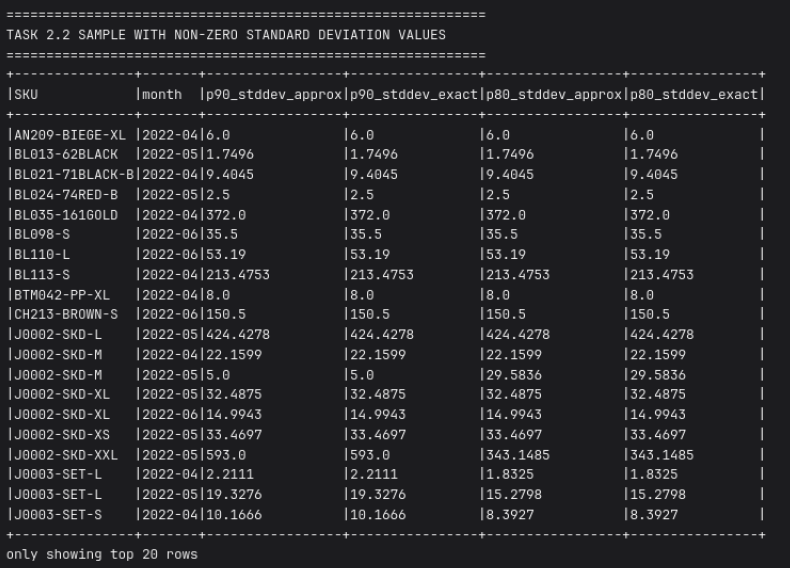
\includegraphics[width=0.9\textwidth]{img/2-2/benchmark.png}
    \caption{Kết quả đo hiệu năng thời gian chạy giữa hai phương pháp}
    \label{fig:task2_2_benchmark}
\end{figure}

\begin{figure}[H]
    \centering
    
\includegraphics[width=0.9\textwidth]{img/2-2/output_preview.png}
    \caption{Một phần nội dung tệp Parquet kết quả đầu ra \texttt{Task\_2-2.parquet}}
    \label{fig:task2_2_output_preview}
\end{figure}
